\documentclass[10pt,a4paper]{article}
\usepackage[T1]{fontenc}
\usepackage{lmodern}
\usepackage[margin=23mm]{geometry}
\usepackage{amsmath,amssymb,booktabs,microtype,pgfplots}
\usepackage[hidelinks]{hyperref}
\pgfplotsset{compat=1.18}
\pdfinfoomitdate=1
\pdftrailerid{}
\pdfsuppressptexinfo=15
\setlength{\parindent}{0pt}
\setlength{\parskip}{5pt}
\title{Hydrogen shell convergence:\\why the atom needs more excited states}
\author{\texttt{exojax-escape}: model definition and verification}
\date{Definition revision 1; 21 November 2026}
\begin{document}
\maketitle

\section{The failure and the physical change}
The previous atom stopped at principal quantum number $N=5$. At the declared
baseline, raising the cutoff from $N=4$ to 5 changed the population of the
$n=3$ shell by $7.735\%$, above the unchanged $5\%$ criterion. Cloudy independently
shows a similar change. This is evidence that the atom is too short: adding a
new shell opens additional recombination, ionization and cascade paths.

\[
\boxed{\text{electrons + protons}}
\ \rightleftarrows\ \boxed{\text{higher shells}}
\ \rightleftarrows\ \boxed{n=3,\ n=2}
\]

The revised model includes every statistical shell through $N\le20$, and uses
$N=15$ as the default. The original six populations remain resolved as
$1s,2s,2p,3s,3p,3d$. A collapsed shell represents all its orbital states by one
population, with fraction $(2\ell+1)/n^2$ in state $\ell$. It retains the summed
physical transition rates; it does not fit a correction factor to $n_2$ or
$n_3$ or add a recombination top-off above the cutoff.

\section{What had to be extended}
Three pieces matter. First, every added shell needs transitions to all lower
retained states. We integrate the finite hydrogenic radial polynomials in
exact rational arithmetic, then convert the final normalized dipole to
float64. This changes how the same nonrelativistic integral is evaluated,
preventing cancellation between very large alternating terms. Construction
happens before the JAX gas-state calculation and introduces no fitted rates.

Second, each shell needs photoionization and its inverse radiative
recombination. The Coulomb-wave cross sections use the Brocklehurst recurrence
already adopted for the smaller atom. We remove a common normalization and
powers of photon energy before the recurrence, and combine radial products
in logarithmic form. Otherwise squaring a very small high-$\ell$ dipole can
underflow before its compensating factors are applied. The physical cross
section and its inverse Milne relation remain the same.

Third, the added $n\ge6$ shells need electron-impact ionization and three-body
recombination. We use the VS80 ionization prescription as implemented in
Cloudy and construct the inverse with the same energy and Saha factor. The
existing $n\le5$ ionization data and the shell bound--bound collision
prescription remain unchanged. Statistical orbital populations and the
collision fits are physical approximations, even when the numerical
implementation passes its checks.

\section{Why the populations change}
Electrons captured into a high shell can reach the lower states through a
cascade. The effect is not an isolated additive source: the new shell also
changes excitation/ionization losses, and the electron density changes when
charge and nucleus conservation are solved again. A retained fixed-electron-
density matrix-elimination calculation separates these terms exactly for
that diagnostic convention. The result supports missing high-shell pathways
as the cause, with both source and charge feedback present. Those components
are a diagnostic decomposition, not independent physical atmospheres.

For the original $4\to5$ change, this diagnostic gives $+2840.7$ cm$^{-3}$
from the added-shell recombination source, $-880.8$ cm$^{-3}$ from the changed
effective rate operator and $-509.4$ cm$^{-3}$ from restored charge feedback.
Their sum, $+1450.5$ cm$^{-3}$, reproduces the $7.735\%$ change. The much larger
opposing terms show why adding a constant cascade correction would miss
part of the response.

The full local model continues to solve statistical equilibrium with
$n_e=n_p$ and $n_p+\sum_i n_i=n_{\rm H}$. The JAX implicit derivative includes
the electron-density dependence of the rates. Both forward and reverse derivatives with respect to gas temperature and
hydrogen density are checked against finite differences, so the
extended atom retains the differentiation needed by later NUTS inference.

\section{What convergence means here}
For shell $s=2$ or 3 we retain the explicit criterion
\[
 \Delta_s(N,N_{\rm ref})=
 \left|\frac{n_s(N_{\rm ref})}{n_s(N)}-1\right|\le0.05.
\]
The new test compares $N=15$ with 20. It also retains the sequence
$5,10,15,20$, continuum-grid refinement and independent Cloudy comparisons.
The old $4\to5$ result stays contradicted: success of a new, larger atom does
not change the answer for the old model.

\begin{figure}[ht]
\centering
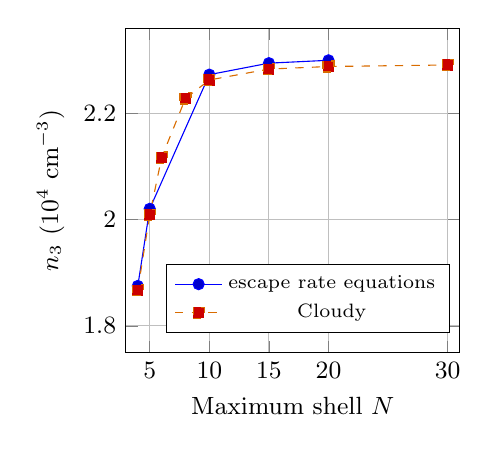
\begin{tikzpicture}
\begin{axis}[width=.48\textwidth,height=5.7cm,xlabel={Maximum shell $N$},
 ylabel={$n_3$ ($10^4$ cm$^{-3}$)},xmin=3,xmax=31,ymin=1.75,ymax=2.36,
 xtick={5,10,15,20,30},legend style={font=\scriptsize,at={(.97,.06)},anchor=south east},
 tick label style={font=\small},label style={font=\small},grid=major]
\addplot+[blue,mark=*] coordinates {(4,1.875228681) (5,2.020277671) (10,2.272697295) (15,2.294308309) (20,2.299665251)};
\addlegendentry{escape rate equations}
\addplot+[orange!85!black,mark=square*,dashed] coordinates {(4,1.867505) (5,2.009105) (6,2.116755) (8,2.227924) (10,2.262646) (15,2.283159) (20,2.287971) (30,2.290882)};
\addlegendentry{Cloudy}
\end{axis}
\end{tikzpicture}\hfill
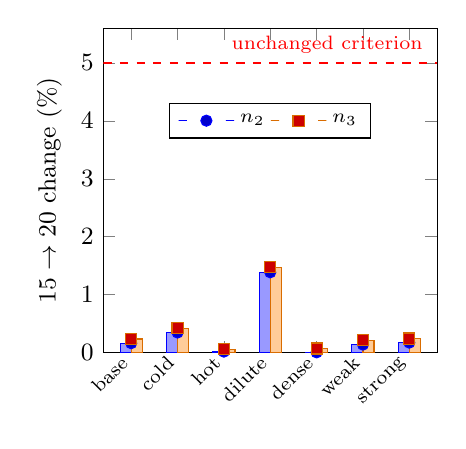
\begin{tikzpicture}
\begin{axis}[width=.48\textwidth,height=5.7cm,ylabel={$15\to20$ change (\%)},
 xmin=.4,xmax=7.6,ymin=0,ymax=5.6,xtick={1,2,3,4,5,6,7},
 xticklabels={base,cold,hot,dilute,dense,weak,strong},
 x tick label style={rotate=45,anchor=east,font=\scriptsize},
 ytick={0,1,2,3,4,5},yticklabel style={font=\small},label style={font=\small},
 legend style={font=\scriptsize,at={(.5,.77)},anchor=north,legend columns=2}]
\addplot+[ybar,bar width=4pt,bar shift=-2pt,blue,fill=blue!40] coordinates {(1,0.1603528851) (2,0.3445587249) (3,0.01509796018) (4,1.384386393) (5,0.002369293216) (6,0.1363045245) (7,0.1705216931)};
\addlegendentry{$n_2$}
\addplot+[ybar,bar width=4pt,bar shift=2pt,orange!85!black,fill=orange!40] coordinates {(1,0.2334883297) (2,0.4171766244) (3,0.05741754658) (4,1.471335027) (5,0.06929931228) (6,0.2107801222) (7,0.2413845907)};
\addlegendentry{$n_3$}
\addplot[red,dashed,forget plot] coordinates {(.4,5)(7.6,5)};
\node[red,anchor=south east,font=\scriptsize] at (axis cs:7.5,5) {unchanged criterion};
\end{axis}
\end{tikzpicture}
\caption{Left: baseline shell sequence. The escape-rate points are independently
solved in the retained matrix-budget diagnosis; the final JAX comparison agrees
at $N=15,20$. Right: actual escape $15\to20$ changes at all seven registered
conditions. These factorized points do not define a continuous accuracy domain.}
\end{figure}

\begin{center}
\begin{tabular}{lll}
\toprule
Comparison & Largest measured difference & Criterion \\
\midrule
Original $4\to5$, baseline $n_3$ & $7.735\%$ & $5\%$: failed \\
New $15\to20$, baseline $n_3$ & $0.2335\%$ & $5\%$: passed \\
New $15\to20$, both populations, seven cases & $1.4713\%$ & $5\%$: passed \\
Matched Cloudy $N=15,20$, fourteen cases & $2.0315\%$ & $5\%$: passed \\
Escape $N=15$ versus selected Cloudy $N=30,40$ & $2.0657\%$ & separate control \\
\bottomrule
\end{tabular}
\end{center}

The baseline uses $T=9000$ K, $n_{\rm H}=10^{12}$ cm$^{-3}$,
$T_{\rm rad}=10000$ K and dilution $W=0.025$. The other conditions change
one quantity: $T=6000$ or $12000$ K, $n_{\rm H}=10^{10}$ or $10^{14}$ cm$^{-3}$,
or $W=0.01$ or $0.05$. The physical criterion remains $5\%$ for both $n_2$ and
$n_3$ in the enlarged-atom comparison. Three Cloudy continuum refinements change
these populations by less than $0.049\%$.


The proposed $N=10$ choice was rejected after the dilute-gas Cloudy control
showed a larger-than-$5\%$ change against $N=20$. The default therefore uses
$N=15$, checked against $N=20$ at the declared cases, with selected larger
Cloudy tails as an additional control. The default is a scoped modeling
choice, not a theorem that fifteen shells suffice everywhere.

\section{MCEG and the remaining limits}
The new contract \path{mceg/contracts/escape.atom_convergence.yaml} records
Equations, source Bindings, the exact tested Subject and Contexts, retained
Evidence and the adoption Decision. It preserves the older contradicted
Assessment and records the new finite comparison separately. Numerical
success, finite-reference agreement and atmospheric adequacy remain distinct.

Only the registered samples are tested; no continuous parameter domain or
infinite-atom limit is established. The high shells still use statistical
orbital populations. The local radiation field is prescribed. Neither this
comparison nor its implicit derivatives validate the full planetary wind,
moving-medium line transfer, an observed H-alpha spectrum or a NUTS posterior.
The runtime package remains independent of MCEG.

\begin{thebibliography}{9}
\bibitem{prozesky} A. Prozesky and D. P. Smits (2018), hydrogenic radiative
coefficients, Appendix A.1, \href{https://arxiv.org/html/1805.02440v1}{arXiv:1805.02440}.
The rational summation used here is a provider implementation choice.
\bibitem{brocklehurst} M. Brocklehurst (1971), \emph{MNRAS} 153, 471,
\href{https://doi.org/10.1093/mnras/153.4.471}{doi:10.1093/mnras/153.4.471},
Eqs.~3.13 and 3.17--3.24; evaluated through the inspected Cloudy recurrence.
\bibitem{vs80} L. Vriens and A. H. M. Smeets (1980), \emph{Physical Review A}
22, 940, \href{https://doi.org/10.1103/PhysRevA.22.940}{doi:10.1103/PhysRevA.22.940}.
Ionization Eq.~8 was inspected in Cloudy's \texttt{hydro\_vs\_ioniz}
implementation; no direct full-text inspection of the paper is claimed.
\bibitem{cloudy} Cloudy C23.01 source and data,
\href{https://data.nublado.org/cloudy_releases/c23/c23.01.tar.gz}{official release}:
\texttt{hydro\_bauman.cpp}, \texttt{hydro\_vs\_rates.cpp}, and
\texttt{data/hydro\_pcs.dat}. The retained license notice and execution
provenance identify the adapted routines and the reference calculations.
\end{thebibliography}

\clearpage
\appendix
\section{Recorded equations and units}
\small
These definitions are generated from the MCEG contract; their source-code
bindings and assessment pins remain in that contract.
% Generated by mceg equations; edit the contract, then regenerate.
% Requires amsmath. Authored math is retained; TeX is not executed here.
% Definitions and hashes do not establish scientific validity.

% equation-sha256: 6c7b52cbfdac3da24c7a52e989f9a6db100292facd652dd3069fabb14dc40a0b
\paragraph{Equation statistical\_shells (revision 1)}
The added shells distribute population statistically over orbital states and sum each physical transition into its destination group.
\begin{equation}
\begin{aligned}
g_n=2n^2,\quad p_{n\ell}=\frac{2\ell+1}{n^2},\\\overline{A}_{nj}=\sum_{\ell=0}^{n-1}p_{n\ell}\sum_{k\in j}A_{n\ell,k},\qquad\overline{\sigma}_n(\nu)=\sum_{\ell=0}^{n-1}p_{n\ell}\sigma_{n\ell}(\nu)
\end{aligned}
\label{eq:escape.atom_5f_convergence:statistical_5f_shells:1}
\end{equation}
\noindent\textbf{Scope:} Resolved 1s,2s,2p,3s,3p,3d; collapsed shells 4 through N, with 3<=N<=20.

\begin{description}
\item[$n$] Principal quantum number (1; ID: principal).
\item[$\ell$] Orbital quantum number (1; ID: orbital).
\item[$g_n,p_{n\ell}$] State degeneracy and orbital population fraction (1; ID: weight).
\item[$A,\overline A$] Spontaneous electric-dipole rate (s\textasciicircum{}-1; ID: einstein\_a).
\item[$\sigma,\overline\sigma$] Photoionization cross section (cm\textasciicircum{}2; ID: cross\_section).
\item[$\nu$] Ordinary photon frequency (Hz; ID: frequency).
\item[$N$] Largest included principal shell (1; ID: maximum\_shell).
\end{description}

\noindent\textbf{Assumptions:}
\begin{itemize}
\item Statistical orbital populations in the collapsed shells are an approximation, not a new resolved high-l kinetic model.
\item Low-level energies and transition rates retain the selected original data.
\item Every retained shell has explicit recombination, ionization and cascade paths; omitted shells have no artificial top-off source.
\end{itemize}

% equation-sha256: b09bb84c99419c1f81e335017fff23cf849deba6cf8ad11ce2a04811249e6373
\paragraph{Equation radial\_dipoles (revision 1)}
Hydrogenic electric-dipole radial integrals; exact rational polynomial integration prevents cancellation in the static construction.
\begin{equation}
\begin{aligned}
\widetilde R_{n\ell}(u)=\frac{2}{n^2}\sqrt{\frac{(n-\ell-1)!}{(n+\ell)!}}e^{-u/n}\left(\frac{2u}{n}\right)^\ell L_{n-\ell-1}^{2\ell+1}\!\left(\frac{2u}{n}\right),\\ d_{n\ell,n^\prime\ell^\prime}=a_{\rm H}\int_0^\infty u^3\widetilde R_{n\ell}(u)\widetilde R_{n^\prime\ell^\prime}(u)\,du,\\ A_{n\ell,n^\prime\ell^\prime}=\frac{64\pi^4 e^2\nu^3}{3hc^3}\frac{\max(\ell,\ell^\prime)}{2\ell+1}d^2_{n\ell,n^\prime\ell^\prime}
\end{aligned}
\label{eq:escape.atom_5f_convergence:radial_5f_dipoles:1}
\end{equation}
\noindent\textbf{Scope:} 1<=n,nprime<=20; n>nprime and |l-lprime|=1 for a downward radiative transition.

\begin{description}
\item[$u=r/a_{\rm H}$] Dimensionless radius (1; ID: radius).
\item[$d$] Radial dipole integral (cm; ID: radial).
\item[$A$] Spontaneous rate averaged over upper magnetic states (s\textasciicircum{}-1; ID: einstein\_a).
\item[$\nu$] Finite-state transition frequency (Hz; ID: frequency).
\item[$n$] Upper principal quantum number (1; ID: n\_upper).
\item[$\ell$] Upper orbital quantum number (1; ID: l\_upper).
\item[$n^\prime$] Lower principal quantum number (1; ID: n\_lower).
\item[$\ell^\prime$] Lower orbital quantum number (1; ID: l\_lower).
\item[$a_{\rm H}$] Protium reduced-mass Bohr radius used by the bound-bound construction (cm; ID: bohr\_radius).
\end{description}

\noindent\textbf{Assumptions:}
\begin{itemize}
\item The Bohr radius uses the declared protium reduced-mass correction.
\item Polynomial summation is exact rational arithmetic; the final normalization and returned rates use float64.
\item This static atomic construction is independent of differentiable gas parameters.
\end{itemize}

% equation-sha256: bbd1bf2e3471abef0371c60714091712293206dbf51bcfc97ccd160674c8de88
\paragraph{Equation coulomb\_bound\_free (revision 1)}
Coulomb-wave cross sections recombine the normalized radial recurrence in logarithmic form.
\begin{equation}
\begin{aligned}
E=\frac{h\nu}{\chi_{n\ell}},\quad t^2=\max(E-1,0),\quad \mathcal E=1+t^2,\quad k=t/n,\\
\log G_* =\tfrac12\log(\pi/2)+\log(8n)+n\log(4n)-\log\Gamma(2n)\\
\hspace{7mm}-2n\frac{\arctan t}{t}-\tfrac12\log(1-\exp[-2\pi/k])-(n+2)\log\mathcal E,\\
\log D_{n\ell,\ell'}^2=\log\frac{(n+\ell)!}{(n-\ell-1)!}
 +\sum_{s=1}^{\ell'}\log(1+s^2k^2)+2(\ell-n)\log(2n)\\
\hspace{7mm}+2[\log G_*+p_\ell^\pm\log\mathcal E+\log|H_\ell^\pm|],\\
p_\ell^+=n-1-\ell,\quad p_\ell^-=n-\ell,\\
\sigma_{n\ell}(\nu)=\frac{4\pi\alpha a_0^2n^2}{3}
 \sum_{\ell'=\ell\pm1\ge0}\frac{\max(\ell,\ell')}{2\ell+1}\,\mathcal E\,\exp(\log D_{n\ell,\ell'}^2)
\end{aligned}
\label{eq:escape.atom_5f_convergence:coulomb_5f_bound_5f_free:1}
\end{equation}
\noindent\textbf{Scope:} 1<=n<=20; cross section zero for E<1. Plus/minus denotes continuum lprime=l+1/l-1. Each finite state uses its actual threshold.

\begin{description}
\item[$n$] Principal quantum number (1; ID: principal).
\item[$\ell$] Bound-state orbital quantum number (1; ID: orbital).
\item[$E$] Photon energy divided by the actual threshold (1; ID: energy).
\item[$G_*,H^\pm,D$] Coulomb radial normalization, normalized recurrence and dipoles (1; ID: radial).
\item[$\sigma_{n\ell}$] Orbital photoionization cross section (cm\textasciicircum{}2; ID: cross\_section).
\item[$a_0$] Bohr radius 5.29177210903e-9 cm used in the bound-free normalization (cm; ID: bohr\_radius).
\end{description}

\noindent\textbf{Assumptions:}
\begin{itemize}
\item At threshold arctan(t)/t tends to one; a small-t series preserves the derivative.
\item Computing the logarithm of the product avoids squaring tiny dipoles before compensating factors are applied.
\item Both photoionization and the inverse Milne process use this same cross section.
\item The support limit n<=20 is explicit; successful tests at sampled energies do not prove an unlimited high-n domain.
\end{itemize}

% equation-sha256: 13b01dd08fb23dad58e64a975e989a47d811317651cc18de0cf86be28e16c893
\paragraph{Equation normalized\_coulomb\_recurrence (revision 1)}
Energy-normalized Brocklehurst recurrence, algebraically equivalent to the earlier unscaled radial recurrence.
\begin{equation}
\begin{aligned}
G_q^+=G_*\mathcal E^{n-1-q}H_q^+,\quad G_q^-=G_*\mathcal E^{n-q}H_q^-,\\
H^+_{n-1}=1,\quad H^+_{n-2}=n(2n-1),\\
H^-_{n-1}=\frac1{2n},\quad H^-_{n-2}=(2n-1)\left(\frac4{\mathcal E}+n-1\right)H^-_{n-1},\\
A_q^+=\frac{4n^2-4(q+2)^2}{\mathcal E}+(q+2)(2q+3),\\
B_q^+=\frac{4n^2[n^2-(q+2)^2][1+(q+3)^2k^2]}{\mathcal E^2},\\
A_q^-=\frac{4n^2-4(q+1)^2}{\mathcal E}+(q+1)(2q+3),\\
B_q^-=\frac{4n^2[n^2-(q+2)^2][1+(q+1)^2k^2]}{\mathcal E^2},\\
H_q^\pm=A_q^\pm H_{q+1}^\pm-B_q^\pm H_{q+2}^\pm
\end{aligned}
\label{eq:escape.atom_5f_convergence:normalized_5f_coulomb_5f_recurrence:1}
\end{equation}
\noindent\textbf{Scope:} Plus runs q=n-3,...,0; minus runs q=n-3,...,1. Initial values are used only when their indices exist. The noncontributing n=1 minus seed is never evaluated as a dipole.

\begin{description}
\item[$n$] Principal quantum number (1; ID: principal).
\item[$E$] Photon energy divided by threshold; the clipped energy is max(E,1) (1; ID: energy).
\item[$k$] Dimensionless continuum momentum (1; ID: continuum).
\item[$H_q^\pm$] Energy-normalized radial factors (1; ID: radial).
\end{description}

\noindent\textbf{Assumptions:}
\begin{itemize}
\item Each downward step removes one power of the clipped photon energy before forming the recurrence.
\item The algorithm is a provider-derived rescaling of the inspected Cloudy/Brocklehurst recurrence, not an empirical population adjustment.
\end{itemize}

% equation-sha256: 022388d9dab1fa55ffdb5170110c0b8d9f123eb7c621395ac556c8f2b87132aa
\paragraph{Equation higher\_shell\_ionization (revision 1)}
VS80 Eq. 8 supplies the added-shell electron ionization rate; its three-body inverse uses the same state energy and statistical weight.
\begin{equation}
\begin{aligned}
u=\frac{k_{\rm B}T}{1\,\mathrm{eV}},\quad\epsilon_n=\frac{\chi_n}{k_{\rm B}T},\\q_n^{\rm ion}=\frac{9.56\times10^{-6}e^{-\epsilon_n}}{u^{3/2}[\epsilon_n^{2.33}+4.38\epsilon_n^{1.72}+1.32\epsilon_n]},\\q_n^{\rm 3b}=q_n^{\rm ion}\frac{g_n}{2}\left(\frac{h^2}{2\pi m_e k_{\rm B}T}\right)^{3/2}e^{\chi_n/(k_{\rm B}T)}
\end{aligned}
\label{eq:escape.atom_5f_convergence:higher_5f_shell_5f_ionization:1}
\end{equation}
\noindent\textbf{Scope:} Only collapsed n=6,...,20 use this extension. The retained n<=5 collision/ionization prescriptions remain distinct.

\begin{description}
\item[$T$] Gas temperature (K; ID: temperature).
\item[$\chi_n$] Actual finite-state ionization threshold (erg; ID: binding).
\item[$q_n^{\rm ion}$] Electron-impact ionization coefficient (cm\textasciicircum{}3 s\textasciicircum{}-1; ID: rate).
\item[$q_n^{\rm 3b}$] Three-body recombination coefficient (cm\textasciicircum{}6 s\textasciicircum{}-1; ID: inverse).
\end{description}

\noindent\textbf{Assumptions:}
\begin{itemize}
\item Maxwellian electrons; the VS80 fit is an adopted approximation.
\item The retained low-level data restrict the shared gas-temperature domain.
\end{itemize}

% equation-sha256: f10a6b3985bb3bf8ef6c50f33864e5d9629a0ac6a6027b056489d7e746796620
\paragraph{Equation finite\_charge\_root (revision 1)}
The retained charge-conserving statistical-equilibrium root is solved for the enlarged rate matrix and differentiated implicitly.
\begin{equation}
\begin{aligned}
P_{ij}=R_{ij}+n_e q_{ij},\quad
 M=\operatorname{diag}\!\left(\sum_jP_{ij}+\Gamma_i+n_e q_i^{\rm ion}\right)-P^{\mathsf T},\\
s_i=n_e\alpha_i+n_e^2q_i^{\rm 3b},\quad b=M^{-1}s,\\
n_e=n_p=n_{\rm H}e^z,\quad n_i=n_e b_i,\quad F(z;\theta)=z+\log(1+\mathbf1^{\mathsf T}b)=0,\\
\frac{dz}{d\theta}=-\frac{\partial_\theta F}{\partial_z F}
\end{aligned}
\label{eq:escape.atom_5f_convergence:finite_5f_charge_5f_root:1}
\end{equation}
\noindent\textbf{Scope:} Pure H, nonnegative finite rates with a positive photoionization rate, nonsingular bound-state matrix, isolated scalar charge root. Gas and radiation inputs are prescribed in this local comparison.

\begin{description}
\item[$n_{\rm H}$] Hydrogen nucleus number density (cm\textasciicircum{}-3; ID: density).
\item[$T$] Prescribed gas temperature (K; ID: temperature).
\item[$n_e=n_p$] Electron and proton density (cm\textasciicircum{}-3; ID: electron).
\item[$n_i$] Bound-state populations (cm\textasciicircum{}-3; ID: population).
\item[$b_i$] Bound-to-proton population ratio (1; ID: ratio).
\item[$P,R,\Gamma,M,s$] Transition rates, loss matrix and source per proton (s\textasciicircum{}-1; ID: rate).
\item[$q_{ij},q_i^{\rm ion},\alpha_i$] Two-body rate coefficients (cm\textasciicircum{}3 s\textasciicircum{}-1; ID: coefficient).
\item[$q_i^{\rm 3b}$] Three-body coefficient (cm\textasciicircum{}6 s\textasciicircum{}-1; ID: three\_body).
\item[$z,F$] Log ionized fraction and conservation residual (1; ID: root).
\end{description}

\noindent\textbf{Assumptions:}
\begin{itemize}
\item Orbital mixing coefficients remain inside the density-dependent rate callback.
\item The implicit derivative follows the converged equations, including rate feedback, rather than differentiating the bisection iterations.
\item The gas-temperature limits of the retained low-level atomic data remain applicable.
\end{itemize}

% equation-sha256: f5c9364243ceecec01d7958d52e8a4f2a56c0157e55df252ff2915c7c2691925
\paragraph{Equation shell\_change (revision 1)}
A sampled relative shell-size criterion with the smaller atom in the denominator.
\begin{equation}
\begin{aligned}
\Delta_s(N,N_{\rm ref})=\left|\frac{n_s(N_{\rm ref})}{n_s(N)}-1\right|,\qquad\max_{s\in\{2,3\}}\Delta_s(15,20)\le0.05
\end{aligned}
\label{eq:escape.atom_5f_convergence:shell_5f_change:1}
\end{equation}
\noindent\textbf{Scope:} The seven registered temperature/density/radiation cases; N=15 and Nref=20. The separate baseline measurement retains 48 points per threshold interval.

\begin{description}
\item[$n_s$] Population summed over resolved sublevels of shell s (cm\textasciicircum{}-3; ID: population).
\item[$\Delta_s$] Absolute relative change on increasing the largest included shell (1; ID: change).
\end{description}

\noindent\textbf{Assumptions:}
\begin{itemize}
\item Each population solve must meet its numerical convergence criteria.
\item Numerical quadrature and derivative tests are separate prerequisites.
\item This finite comparison cannot establish infinite-atom convergence or physical atmospheric accuracy.
\end{itemize}

\end{document}
